\section{The $\nu$PRISM detector concept \label{sec:nuprism}}
The concept for the $\nu$PRISM detector is illustrated in Fig.~\ref{fig:nuprism_concept}.  It is a tall water-Cherenkov 
detector located 1-2~km from the neutrino source in J-PARC neutrino beam.  At 1~km, the detector is $\sim$50~m tall, covering
the off-axis angle range of 1-4 degrees. The base-line to the detector is set to at least 1~km to control event pile-up rates
and to reduce the line source effect of the pion beam.  A water-Cherenkov detector is chosen since measurements on H$_{2}$O are
most relevant for T2K and Hyper-K and the detector technology scales to large fiducial masses well.  The detector diameter is 
set to 10~m based on the need to contain forward going muons with momentum up to 1.5 GeV/c to probe the relevant phase space for
T2K and Hyper-K.  More details of the design considerations and construction techniques for $\nu$PRISM are given in 
Section~\ref{sec:nuprism_build}.

In $\nu$PRISM, a new off-axis angle, $\theta_{OA}$ observable is introduced.  This observable is estimated by using the reconstructed
vertex position for each event in $\nu$PRISM and calculating the angle between the average beam direction and the vector from the 
average neutrino production point to the reconstructed vertex.  A given $\theta_{OA}$ corresponds to a predicted neutrino spectrum,
and this additional information can be used to overconstrain the cross-section models or derive cross-sections in a model independent
way.

\begin{figure}
 \begin{center}
  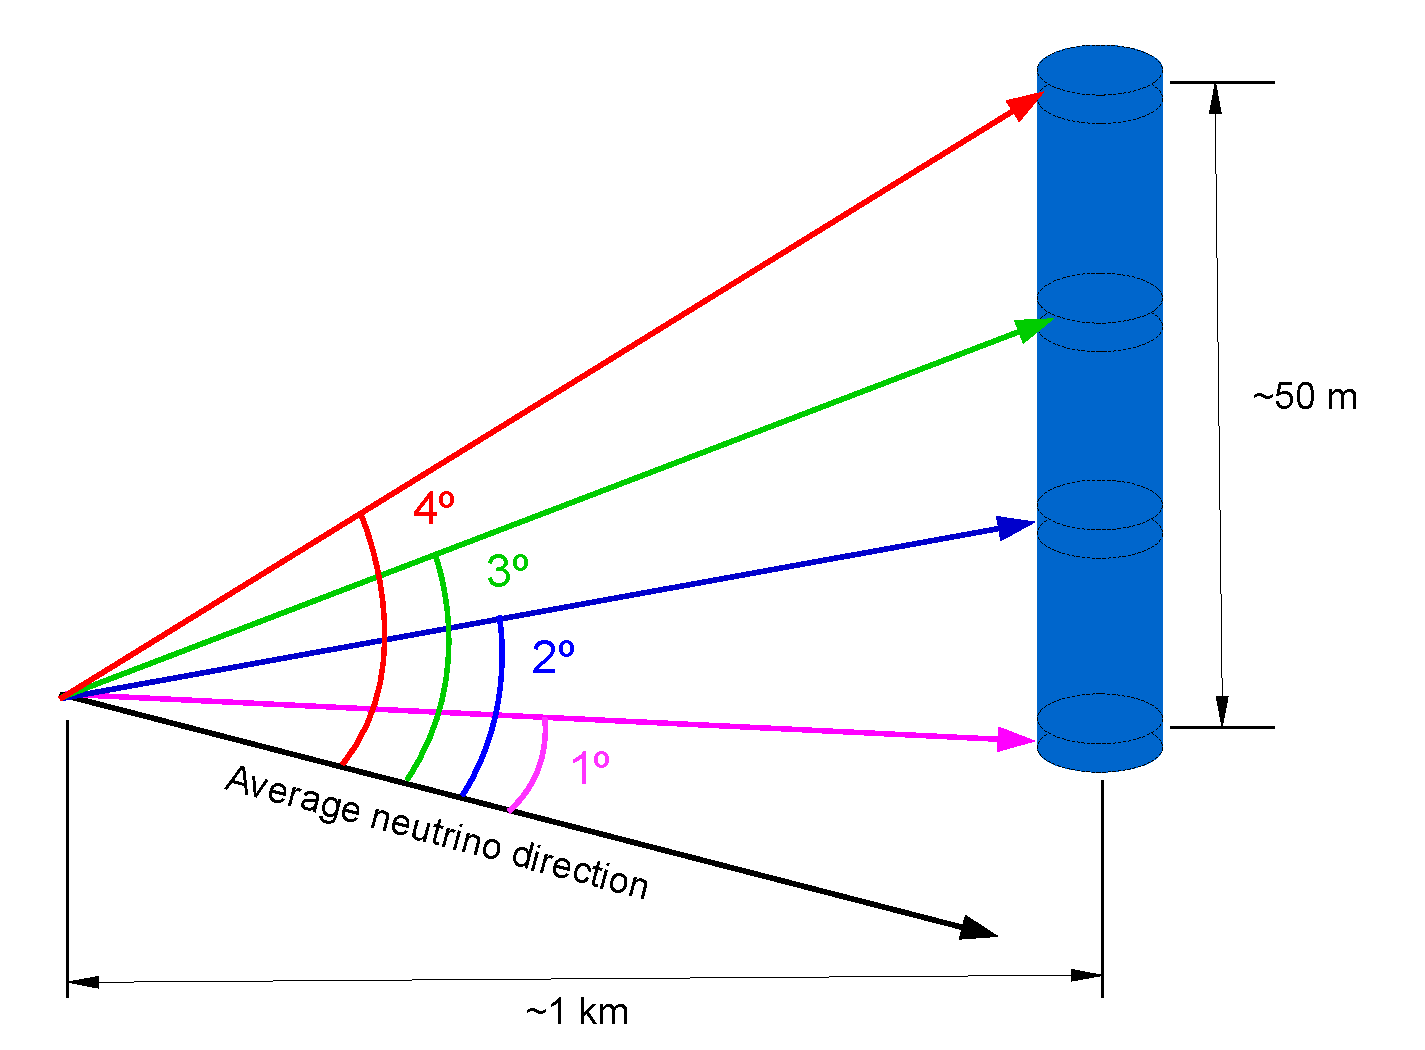
\includegraphics[width=0.85\textwidth]{figures/nuprism_schematic.pdf}
  \caption{The $\nu$PRISM detector concept.}
  \label{fig:nuprism_concept}
  \end{center}
\end{figure}

\subsection{Measurments in $\nu$PRISM}
Charged current muon and electron neutrino interactions in $\nu$PRISM are identified by observing Cherenkov rings that
are consistent with penetrating or showering particles respectively.  Muon and electron candidates are further separated by the
presence of a delayed Michel electron from the muon decay.  Events with a single prompt muon or electron candidate ring are 
used for the oscillation candidate samples in T2K or Hyper-K oscillation measurements.  Table~\ref{tab:events} shows the number
and purity of these events in $\nu$PRISM at 1~km with a 1e21 proton-on-target exposure.

\begin{table}[tbh]
\caption{The $\nu$PRISM candidate event rates for single ring muon and electron like samples for 1e21 protons on target in
the J-PARC beam.}
\label{tab:events}
\begin{tabular}{l|cc|cc}
\hline
Off-axis Range & 1 Ring Muon Candidates & CC $\nu_{\mu}$ Purity & 1 Ring Electron Candidates & CC $\nu_{e}$ Purity \\
\hline
1$^{\circ}$-2$^{\circ}$ & 7.8e5 & 97.3\% & 5.4e3 & 32.5\%\\
2$^{\circ}$-3$^{\circ}$ & 4.3e5 & 97.7\% & 4.5e3 & 51.8\% \\
3$^{\circ}$-4$^{\circ}$ & 1.9e5 & 97.2\% & 2.9e3 & 65.0\% \\
\hline
\end{tabular}
\end{table}

The $\nu_{\mu}$ neutrino statistics and purity are high enough that the final state particle response can be derived for 
an almost arbitrary input spectrum using the information from the various off-axis spectra.  For example, the final state
muon momentum and scattering angle distributions for a nearly mono-energetic spectrum or an oscillated spectrum can 
be derived, as described in Section~\ref{sec:nuprism_numu}.

The $\nu_{e}$ statistics and purities in Table~\ref{tab:events} are derived using the same photo-coverage (40\%) and 
PMT size (20~inch) as Super-Kamiokande.  As was shown in the proposal for a 2~km water Cherenkov detector for T2K, smaller
PMTs with finer granularity can improve the performance, and that approach is being investigated for $\nu$PRISM. 
Regardless,
even with 1e21 protons on target and large PMTs, a measurement of the $\nu_{e}$ cross section with a 3\% statistical uncertainty
on the normalization is possible.  The $\nu_{e}$ candidate events will be used to measure the cross-section ratio relative to 
CC $\nu_{\mu}$ interactions and to search for short baseline $\nu_e$ appearance, as described in Section~\ref{sec:nuprism_numu}.

It is also possible to reconstruct events with two or more rings in $\nu$PRISM.  Events with a lepton candidate and additional 
charged particle ring can be used to measure the cross-section for single charged pion production in charged current interactions.
Events with two rings consistent with showering particles may be reconstructed as NC$\pi^{0}$ events, and events with a muon-like
particle that undergoes a hadronic scatter can be reconstructed as NC$\pi^{\pm}$ events.   For the neutral current events,
$\nu$PRISM provides a unique opportunity to directly measure the energy dependence of the cross-section in a single experiment.
These additional measurements with $\nu$PRISM are described in Section~\ref{sec:nuprism_other}.

\subsection{Flux modeling for $\nu$PRISM}
$\nu$PRISM takes advantage of the off-axis angle observable $\theta_{OA}$ to predict the underlying neutrino spectrum
for each interaction in $\nu$PRISM.  The predicted spectrum is based on the flux model.  For T2K the flux is predicted
based on a data-driven simulation of the neutrino beamline from the interaction of protons in the target to the decay of
hadrons and muons that produce neutrinos~\cite{Abe:2012av}.  The dominant uncertainties in the flux modeling arise from
modeling of hadronic interactions in the target, the magnetic horns and the decay region walls.  However, dedicated 
measurements from hadron production experiments such as NA61/SHINE are significantly reducing these uncertainties.  
These hadron production measurements include measurements of particle production multiplicities on replica targets.
By fully incorporating the replica target data, it is expected that experiments will be able to reduce uncertainties on the
flux prediction even lower than the $\sim10\%$ that has already been achieved by T2K and MiniBooNE~\cite{AguilarArevalo:2008yp}.  
With a precise 
flux prediction for $\nu$PRISM, the dependence of the neutrino spectra on $\theta_{OA}$ can be determined independently 
from $\nu$PRISM measurements, and that information can be incorporated in the derivation of neutrino cross-sections from the
$\nu$PRISM data. 
